% !TEX root = main.tex
We consider an offline scenario, which means we know all $t_i$'s and $\ETx_i$'s, non causally. We assume that the receiver harvests energy only once at time $r_0=0$. Hence, the receiver (and so does the transmitter) can be \textit{on} for a maximum period of $\TRx_0$. We also assume that an infinite battery capacity is available both at the transmitter and receiver to store the harvested energy. Our objective is to complete transmission (transmit $B_0$ bits) as early as possible. This is stated as an optimization problem below.

%The transmitter is supposed to transmit all $B_0$ bits in as minimum time as possible. The problem is formally stated below.
\begin{problem}
\begin{align}
&\min_{\{\textbf{p},\textbf{s},N\}}			&& T
\\
&\text{subject to} 				&& B(T)=B_0, 
\label{pb1_constraint_bits}
\\
&     										&& U(t)\le \mathcal{E}(t)  		&&& \forall \; t\;\in\;[0,T], \label{pb1_constraint_energy}
\\
&    										&& s_{N+1}-s_1\le \mathcal{R}_0.
\label{pb1_constraint_time}
\end{align}
\end{problem}
Before describing an algorithm to solve Problem 1, we state the following Lemmas, which shall help us construct our algorithm.
\begin{lemma}
The transmitted power in a optimal solution in non-decreasing with time whenever the receiver is \textit{on}.
\label{increasing_power}
\end{lemma}
\begin{proof}
We prove this by contradiction. Assume that the transmit power is $p_1$ for some duration $t_1$ and then $p_2$ for some duration $t_2$ with $p_1>p_2$. So this boils down to two cases-

$case-1:$ The receiver is on throughout time $t_1$ to $t_2$ as shown in figure. In this case suppose we transmit at a power $p'=\dfrac{p_1t_1+p_2t_2}{t_1+t_2}$ then the number of bits transmitted would be more over the same time duration due to concavity of $g(p)$ as shown below.
\begin{align}
&g(p_1)\frac{t_1}{t_1+t_2}+g(p_2)\frac{t_2}{t_1+t_2} \le g(\frac{p_1t_1+p_2t_2}{t_1+t_2})
\\
&\implies g(p')(t_1+t_2)\ge g(p_1)t_1+g(p_2)t_2  
\end{align}
As we can transmit more number of bits during duration $t_1+t_2$ we could save total transmition time since we would have lesser number of bits left to transmit. Hence this case cannot be optimal.

$case-2:$ The receiver is \textit{off} for certain duration (say $t$) of time during $t_1+t_2$ as shown in figure. Now consider the case where keeping everything else intact we put the receiver \textit{off} from instant $A$ to $A+t$ and keep transmition from $A+t$ to $A+t_1+t_2$. This would always be feasible from the receiver point as energy with the receiver can only be non-decreasing with time. This scenario now boils down to $case-1$ from time $A+t$ to $A+t_1+t_2$ and hence cannot be optimal.
\end{proof}

\begin{lemma}
In a optimal solution once transmition has started the receiver is never \textit{off} until transmition is complete. \label{nobreaks}
\end{lemma}
\begin{proof}
This is equivalent to saying there is no-breaks during transmition in optimal solution. We again prove this by contradiction. Keeping intact Lemma \ref{increasing_power} the only case in which this can occur is the transmitter transmits with power $p_1$ from time $A$ to $B$ and then the receiver is \textit{off} from $B$ to $C$, again the transmitter is \textit{on} with power $p_2$ from time $C$ to $D$ with $p_1<p_2$ as shown in figure . Consider the case where we keep the receiver \textit{on} for time $C-B$ from $A$. This makes the scenario as shown in figure . Now, a new energy arrival can occur at the transmitter anywhere between $A$ to $D$. 

$case-1:$If the arrival is between $A$ and $B'$, then it can be easily seen that transmitting at a constant rate from $B'$ to $D$ would be better due to concavity of $g(p)$.

$case-2:$If the arrival is between $B'$ and $C$ (say $C'$), then it can be easily seen that transmitting at a same rate $p_1$ from $B'$ to $C'$ and  at a constant rate from $C'$ to $D$ would deliver more number of bits.(At worst case energy arrival occurring at $C$ would make this scenario transmit equal number of bits as the original scenario).

$case-3:$If there is an energy arrival from $C$ to $D$ (say $D'$), then transmitting at a constant power form $B'$ to $D'$ and at same rate $p_2$ would fetch more number of bits at the receiver.

Applying the above scenarios iteratively we could shift the receiver \textit{off} duration $C-B$ to the beginning of transmition and still at worst case transmit equal number of bits in same time duration. Hence having a break in-between transmition is always discouraged. We can also see that the optimal solution may not be unique.
\end{proof}

\begin{lemma}
In the optimal solution we consider transmit power can only change at energy arrival of transmitter once transmission has started. 
\end{lemma}
\begin{proof}
Keeping in mind Lemma \ref{increasing_power} and \ref{nobreaks} its proof becomes same as the one for Lemma 2,[]. 
\end{proof}
% !TEX root = OptimalOffline.tex

Concluding the results of Lemmas \ref{lemma_increasing_power}-\ref{transmission_duration}, the optimal policy $\{\textbf{p},\textbf{s},N\}$ must change transmission powers (if any) at energy arrival epochs only i.e. $\forall 1<i<N+1,\ s_i=t_j$ for some $j$. At these epochs, it exhausts the total energy available i.e. $U(s_i)=\ETx(s_i^-)$. The transmission powers are also non decreasing with time. The policy exhausts the total 'receiver time' time allowed, if it does not start transmitting from origin.

Now that we have gained some knowledge of the structure the optimal policy has to follow, we consider an example to approach Problem 1. 

Suppose we are given that the receiver can be \textit{on} for a maximum duration of $\TRx_0$. Our goal is to find a transmission policy so that we can minimize the time at which the transmission is completed. To do this, we shall first find a feasible solution i.e. one which satisfies all constraints (\ref{pb1_constraint_bits})-(\ref{pb1_constraint_time}) and keep improving upon it, until we have a solution that follows all our Lemma \ref{lemma_increasing_power}-\ref{transmission_duration} and hits the boundary on some or all of the constraints (\ref{pb1_constraint_bits})-(\ref{pb1_constraint_time}). 

We need an initial feasible solution to begin with. For this, we find the minimum energy required by the transmitter so that the transmission can be completed in duration $\TRx_0$ with a constant power. That is, the first $\ETx(t_n)$ such that
\begin{equation}
\TRx_0 g\left(\frac{\ETx(t_n)}{\TRx_0}\right)\geq B_0.
\end{equation}
Let $\widetilde{\TRx}_0$ be the time duration such that
\begin{equation}
\widetilde{\TRx}_0 g\left(\frac{\ETx(t_n)}{\widetilde{\TRx}_0}\right)=B_0.
\end{equation}
Let $p_c=\frac{\ETx(t_n)}{\widetilde{\TRx}_0}$. We try to transmit with this power starting at time $t=0$. If it does not violate the energy constraint (\ref{pb1_constraint_energy}), we are done with the optimal solution and our transmission is completed in $\widetilde{\TRx}_0$ time.

If not, we start the transmission as early as possible, such that the transmission is feasible with respect to (\ref{pb1_constraint_energy}). This transmission policy, will encounter atleast one epoch where total energy consumed till that epoch is equal to the total energy harvested upto it. Let time $t_q$ be the first point where this happens. This is shown in Fig. \ref{straight} (a).  Till now we have not argued why we chose such a policy to start with. In fact the Lemma \ref{lemma_Q} shows that this starting solution is a 'good' estimate of policy at and before time $t_q$, as both the optimal policy and the above policy run out of all their energy at epoch $t_q$. 

Now, according to Lemma \ref{lemma_energy_consumed}, the optimal policy must finish all available energy when it stops transmission. If transmitting with $p_c$ power does use up all the energy (Fig. \ref{straight} (b)), then we accept the constant power transmission with $p_c$ as our initial policy (line number \ref{init_policy_CP} in Algorithm \ref{init_policy}). If it does not finish up all of $\ETx(t_n)$ with $p_c$ power till the end (shown in Fig. \ref{straight} (b)), we should choose a better policy after time $t_q$. Let $p_c$ sends $\widetilde{B}$ amount of bits after $t_q$, which is calculated in line number \ref{init_policy_bits_t_q} of INIT\_POLICY. Now, we require our transmission policy to send $\widetilde{B}$ bits after time $t_q$, in as little time as possible (and of course, before $S$), keeping in mind that the policy should use all $\ETx(t_n)$ amount of energy till the end. Algorithm 1 in \cite{Yang} does the job for us. Hence in this case, we choose transmission with $p_c$ till $t_q$ and then the solution of Algorithm 1 in \cite{Yang} after time $t_q$. 

\begin{figure}
\centering
  \centerline{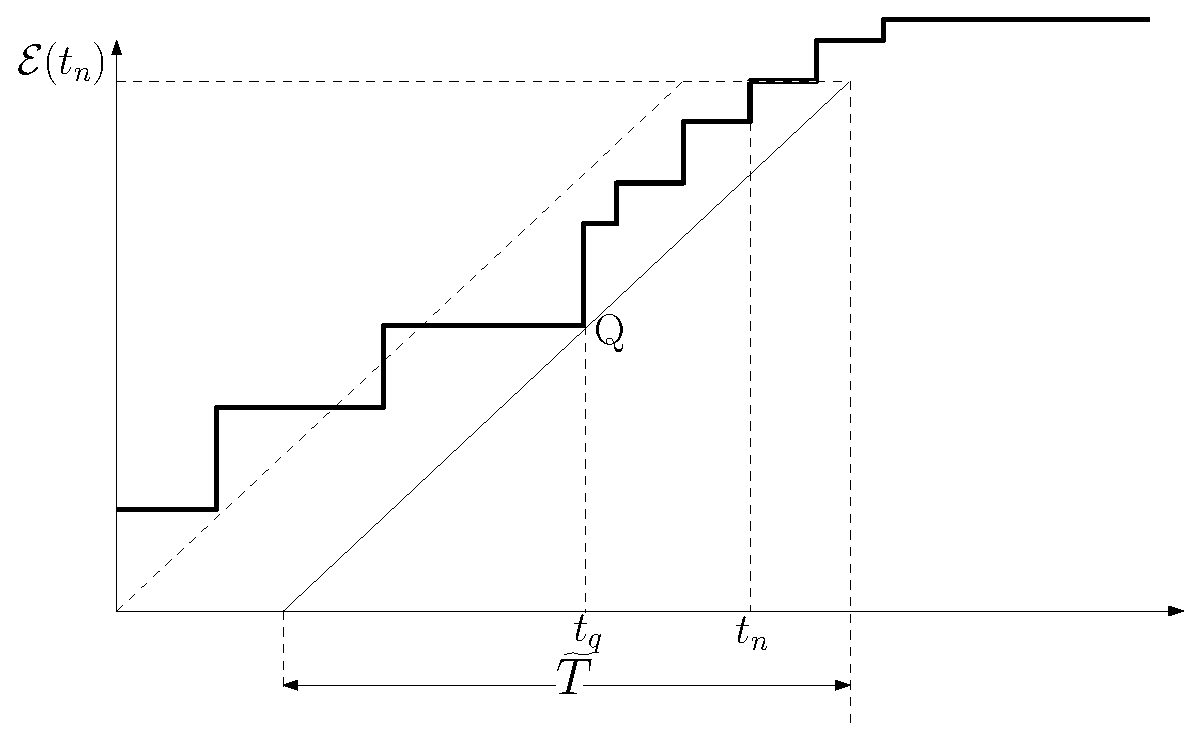
\includegraphics[width=8cm]{straight.eps}}
\caption{Figure showing point $t_q$.}\label{straight}
\end{figure}

\begin{lemma}
In every optimal solution, at energy arrival epoch $t_q$, $U(t_q)=\ETx(t_q^-)$.
\label{lemma_Q}
\end{lemma}
\begin{proof}
We shall prove this by contradiction. Let the start and end times of the constant power transmission policy $p_c$ be $R$ and $S$ receptively. We make the following claims:

\textbf{Claim 1:} Every optimal transmission policy begins transmission at or before time $R$.

Since, $S-R=\widetilde{\TRx}_0\le \TRx_0$, by Lemma \ref{transmission_duration}, if a transmission policy has to finish before $S$, it has to start before time $\max(S-\TRx_0,0) \le \max(R,0)=R$. 

%Since we are transmitting all the bits at the maximum possible power, no policy that starts after $R$ can finish before $S$. Therefore, any policy that starts after $R$ cannot be optimal.

\textbf{Claim 2:} Every optimal transmission policy ends transmission at or before time $S$.
This follows immediately from the fact that the policy is optimal.

%Let $t_q$ equal to time $t_i$ for some $i\in\mathbb{N}$. 
Suppose we have an optimal transmission policy that does not exhaust all its energy at time $t_q$ i.e. $U(t_q)<\ETx(t_q^-)$. By Lemma \ref{lemma_energy_consumed}, it does not change its transmission power at $t_q$. Let the transmission power of optimal policy be $p$ at $t_q$. This does not change till an epoch, say $t_j$. Now, $t_j<S$ by \textit{Claim 2}. Further, power $p_c$ exhausts all energy by $t_q$. So,
\begin{align}
&p_c(t_i-R)=\ETx(t_q^-)\label{eqlemmaQ1}.
\end{align}
But, by constraint (\ref{pb1_constraint_energy})
\begin{align}
&p_c(t_q-R)+p_c(t_j-t_q)\le \ETx(t_j^-),
\\
&\implies p_c(t_j-t_q)\stackrel{(\ref{eqlemmaQ1})}{\le} \ETx(t_j^-)-\ETx(t_q^-),\\
&\implies p_c(t_j-t_q)< \ETx(t_j^-)-U(t_i)=p(t_j-t_q),\\
&\implies p_c<p .\label{eqlemmaQ2}
\end{align}
If the optimal policy does have a power higher than $p_c$ at $t_q$, then it must have the same power of transmission either from some epoch, say $t_k$, or from the beginning of transmission. If $t_k>R$, we can show that $p_c$ becomes infeasible with respect to energy constraint (\ref{pb1_constraint_energy}) at $t_k$. If $t_k<R$, $p$ becomes infeasible with energy constraint \eqref{pb1_constraint_energy} at time $R$. Now, only thing left is the optimal policy begins transmission with power $p$. If so, then it has to begin transmission after time $R$ which follows from equation (\ref{eqlemmaQ2}). This violates \textit{Claim 1}. Therefore every optimal transmission policy must use all energy till epoch $t_q$.
\end{proof}

Now that we have a starting feasible solution, we shall proceed to improve upon this policy as follows. The formal algorithm is presented as Algorithm \ref{Algorithm1}. In any iteration, let $t_{l}$ and $t_{r}$ be the first and last energy arrival epochs where the power of transmission changes. $p_l$ and $p_r$ are the first and last power. The policy found by the Algorithm in-between time $t_l$ and $t_r$ is stored in array \textbf{p} and \textbf{s}. The possible cases that can happen in an iteration of the Algorithm are shown in Fig. \ref{figure_Algorithm1}. 

Step1: The Algorithm tries to increase $p_r$ as much as possible till it hits the boundary of energy constraint \eqref{pb1_constraint_energy} as shown in Fig. \ref{figure_Algorithm1}(a). Then the Algorithm calculates the possible power $p_l'$ such that it transmits same number of bits in total with the previous iteration policy as shown in line number \ref{algo_bits_left_1} and \ref{algo_bits_left_2} of Algorithm \ref{Algorithm1}. 

Step2: If $p_l'$ is feasible, which is the case shown in Fig. \ref{figure_Algorithm1}(a), the policy changes $p_l$ to $p_l'$ and $p_r$ to $p_r'$ (with $t_r$ to $t_r'$). $T_{start}$ and $T_{stop}$ are changed accordingly. 

Step3: If $p_l'$ is not feasible, as shown in Fig. \ref{figure_Algorithm1}(b), then $p_l'$ is set to be the maximum possible feasible power from $t_l$, as shown in Fig. \ref{figure_Algorithm1}(c). Now, $p_r'$ is recalculated so as to settle the transmission of equal number of bits as the previous iteration. We can be sure that $p_r'$ calculated now, would not be infeasible. In this case $t_l$ gets updated to $t_l'$ rather than $t_r$.  

Going back to the first step of the algorithm where we were increasing $p_r$, it could happen, as shown in Fig. \ref{figure_Algorithm1}(d), that $p_r$ goes to infinity without violating the energy constraint \eqref{pb1_constraint_energy}. This happens when there is no energy epoch between $t_r$ and $T_{stop}$. In this scenario, transmission is stopped at $t_r$,i.e. $T_{stop}$ gets updated to $t_r$ and both $t_r$ and $p_r$ are set to the last values in array \textbf{s},\textbf{p} receptively. This is shown in Fig. \ref{figure_Algorithm1}(d). Now, the Algorithm proceeds to calculate $p_l'$ as done in Step1, and continues as before to check whether $p_l'$ is feasible and decides accordingly.

\begin{figure}
\centering
  \centerline{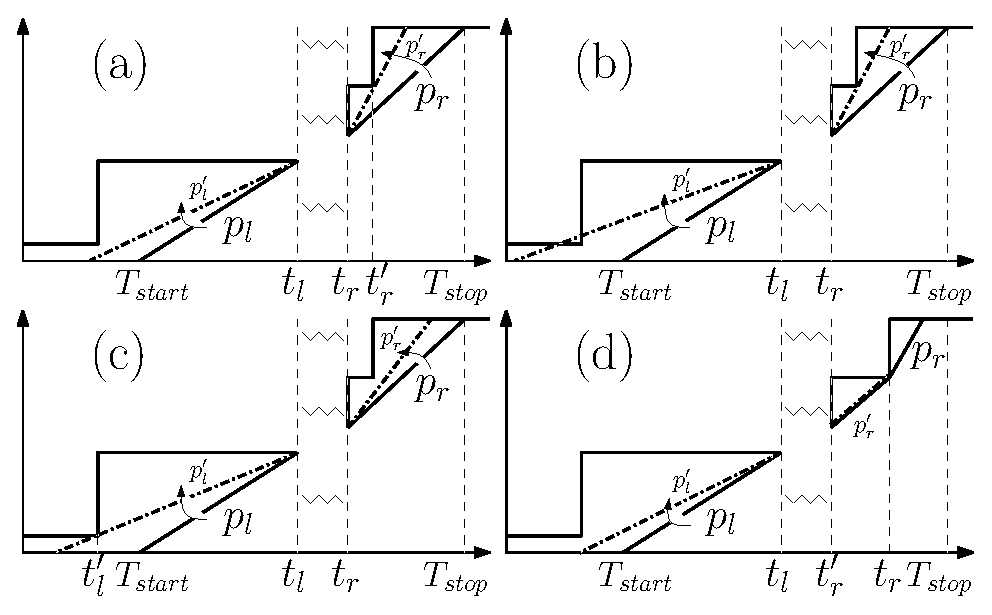
\includegraphics[width=8cm]{Algorithm1.eps}}
\caption{Figures showing any iteration of the Algorithm \ref{Algorithm1}. The solid line represents the transmission policy in the previous iteration. The dash dotted lines in (a), (b), (c), (d) represent the possible configurations of policy in the current iteration.}\label{figure_Algorithm1}
\end{figure}

This is how the algorithm proceeds to generate a new transmission policy in every iteration, which begins and ends earlier than the policy given by the previous iteration, until a point is reached where either $T_{stop}-T_{start}>\TRx_0$ or $T_{start}=0$. Suppose the Algorithm terminates with $T_{start}=0$ and $T_{start}-T_{stop}\le\TRx_0$, then the policy at this iteration is the optimal policy. 


For the case where the algorithm terminates with $T_{stop}-T_{start}>\TRx_0$, let $T_{start}'$, $T_{stop}'$, $p_l'$, $p_r'$, $t_l'$, $t_r'$ be the values in the termination iteration and $T_{start}$, $T_{stop}$, $p_l$, $p_r$, $t_l$, $t_r$ be the values in the previous iteration. Then, the possible valid configurations can be one of the three shown in Fig. \ref{figure_Algorithm1} (a) (c) (d). Note that $\ETx(T_{stop}^-)=\ETx(T_{stop}'^-)$ in all the cases. (In case Fig. \ref{figure_Algorithm1} (d) we can assume that $T_{stop}'=t_r^+$ and transmission exists after $t_r$, but with infinite power. Since transmitting with infinite power for $0$ time does not transmit any bits, we would transmit the same number of bits, as we did prior to this modification). Thus, by Lemma \ref{lemma_increase_time}, we can verify that $(T_{stop}'-T_{start}')>(T_{stop}-T_{start})$. Since $(T_{stop}'-T_{start}')>\TRx_0>(T_{stop}-T_{start})$, there must exist a solution to equation presented in line number \ref{algo_solve_eqn} of Algorithm \ref{Algorithm1}. Let the policy obtained from the solution start and end at $T_{start}''$ and $T_{stop}''$. Then $T_{stop}''$ and $T_{start}''$ would lie in-between $T_{stop}$,$T_{stop}'$ and $T_{start}$,$T_{start}'$ respectively. Also, $T_{stop}''-T_{start}''=\TRx_0$.

So we can conclude by stating that, the solution to Algorithm \ref{Algorithm1} satisfies Lemma \ref{lemma4}. Now, according to the definition of $t_n$ and $t_q$ in line number \ref{init_policy_Etn} and \ref{init_policy_t_q} of INIT\_POLICY, $t_q\le t_n$ and $\ETx(t_q)<\ETx(t_n)$. Since $t_n$ is defined as the first energy arrival epoch by which $B_0$ bits can be transmitted in $\TRx_0$ time, any transmission policy which ends at of before $t_n$ should take more than $\TRx_0$ time to transmit all of $B_0$ bits. As $t_q\le t_n$, we are guaranteed that no transmission policy can finish at or before $t_q$. Hence in the iterations of the algorithm $t_r$ can never decreases beyond $t_q$. Therefore, $t_q$ always exists in the final solution to Algorithm \ref{Algorithm1}.   

%!TEX root = OptimalOffline.tex
%input{Siddhartha}
\begin{theorem}
A transmission policy $\{\textbf{p},\textbf{s},N\}$ is an optimal solution to Problem 1 if and only if it satisfies the following structure.
\label{th_algo1_1}
\begin{align}
&\sum_{i=1}^{i=N}g(p_i)(s_{i+1}-s_i)=B_0; 								
\label{claim1}
\\
&\nonumber s_{N+1}-s_1=\mathcal{R}_0, 	 \ \ \ \ 						\text{ if } s_1>0 \text{ or }
\\
& s_{N+1}\le \mathcal{R}_0,				\ \ \ \ \ \ \ \ \ \				\text{ if } s_1=0;
\label{claim2}
\\
& \nonumber s_{n+1}=\argmin_{t_i: s_n < t_i \le s_{N+1}} \mathcal{P}(s_n,t_i)=\dfrac{\ETx(t_i^-)-U(s_n)}{t_i-s_n} \	\text{ and }
\\
&p_n=\mathcal{P}(s_{n},s_{n+1});\label{claim3}							
\\
&\exists s_j:s_j\in \textbf{s} \text{ and } s_j=Q.					
\label{claim4}
\end{align}
for $n=\{ 1,2,..,N\}$.
\end{theorem}
\begin{proof}
The proof consists of establishing both necessary and sufficiency conditions. First we work out the necessary part i.e. a optimal policy $\{\textbf{p},\textbf{s},N\}$ must have the given structure. We prove it by contradiction. We establish structure (\ref{claim3}) at first. Assume the optimal policy $\{\textbf{p},\textbf{s},N\}$ satisfies Lemmas 1-5 and does not satisfy structure (\ref{claim3}). Specifically, say the policy abides by the  structure (\ref{claim3}) from time $s_{1}$ to $s_n$, for some $n\in \{1,2,..,N\}$ but transmission power right after $s_n$ is not the minimum feasible constant power, i.e.
\begin{align}
p_n>\mathcal{P}(s_n,\tilde{s})\text{ where } \tilde{s}=\argmin_{t_i: s_n < t_i \le s_{N+1}} \mathcal{P}(t_i,s_n).\label{claim3_1}
\end{align}
Note that $p_n\nless \mathcal{P}(s_n,\tilde{s})$ as $\mathcal{P}(s_n,\tilde{s})$ is the minimum feasible power among all the epochs. The maximum energy that can used for transmission from time $s_{n}$ to $\tilde{s}$ is $\left(\ETx(\tilde{s}^-)-\ETx(s_{n}^-)\right)$, since the policy has used all the energy till time $s_{n}^-$, by Lemma \ref{lemma_energy_consumed}. If $\tilde{s}<s_{n+1}$, the transmission policy uses $p_n(\tilde{s}-s_{n})$ energy from time $s_n$ to $\tilde{s}$. If $\tilde{s}>s_{n+1}$, the transmission power during time $[s_{n+1},\tilde{s}]$ has to be greater than or equal to $p_n$ by Lemma \ref{lemma_increasing_power}. So the total energy used during period $[s_n,\tilde{s}]$ can be lower bounded by $p_n(\tilde{s}-s_{n})$. But, this energy is always more than the maximum energy available from $s_{n}$ to $\tilde{s}$ because
\begin{align}
&\nonumber\ETx(\tilde{s}^-)-\ETx(s_{n}^-)=\mathcal{P}(s_n,\tilde{s})(\tilde{s}-s_{n})<p_n(\tilde{s}-s_{n}),
\end{align}
where the inequality follows from (\ref{claim3_1}). This violates constraint (\ref{pb1_constraint_energy}) and contradicts the optimality of policy $\{\textbf{p},\textbf{s},N\}$.
 
Moving on to other structures, (\ref{claim1}) must be followed by the optimal policy as it is a constraint to the Problem 1 and (\ref{claim4}) follows from Lemma 5. We are left to prove structure (\ref{claim2}). $s_{N+1}-s_1\le \mathcal{R}_0$ by constraint (\ref{pb1_constraint_time}). If $s_1=0$ then we are done. When $s_1>0$, assume that $s_{N+1}-s_1<\mathcal{R}_0$. Now consider the policy where power vector is given by $\bm{\widetilde{p}}=\{p_1-\alpha,p_2,..,p_{N-1},p_N+\beta \}$ and the corresponding time vector be given by $\bm{\widetilde{s}}=\{s_1-\gamma,s_2,..,s_{N},s_{N+1}-\delta\}$, where $\gamma=\dfrac{\alpha}{p_1-\alpha}(s_2-s_1)$, $\delta =\dfrac{\beta}{p_N+\beta}(s_{N+1}-s_N)$ and $\alpha ,\beta$ are small positive constants. Since $(s_{N+1}-\delta)>s_{N+1}$, this policy finishes before the optimal policy $\{\textbf{p},\textbf{s},N\}$ and hence amounts to a contradiction only if we are able to show that it is feasible. By the definition of $s_i$ in (\ref{claim3}), $s_{2}$ is the first energy arrival which is on the boundary of energy constraint (\ref{pb1_constraint_energy}) i.e. $U(s_2)=\ETx(s_2^-)$ and $s_{N}$ is the last epoch satisfying $U(s_N)=\ETx(s_N^-)$. So we can choose arbitrarily small $\alpha ,\beta$ such that policy $\{\bm{\widetilde{p}},\bm{\widetilde{s}},N\}$ would be feasible with respect energy constraint (\ref{pb1_constraint_energy}). For every $\beta\rightarrow 0^+$ we can find a value of $\alpha$ such that the number of bits transmitted in policy $\{\bm{\widetilde{p}},\bm{\widetilde{s}},N\}$ remains the same as policy $\{\textbf{p},\textbf{s},N\}$ i.e. equal to $B_0$. So, excluding the common parts in the transmission policy $\{\textbf{p},\textbf{s},N\}$ and $\{\bm{\widetilde{p}},\bm{\widetilde{s}},N\}$, we can equate
\begin{align}
&g(p_N)(s_{N+1}-s_N)+g(p_1)(s_2-s_1)\nonumber
\\
&=g(p_1-\alpha)(s_2-s_1+\gamma)+g(p_N+\beta)(s_{N+1}-s_N-\delta)\nonumber,
\\
&\implies \delta(p_N+\beta)p_N\frac{1}{\beta}\left(\frac{g(p_N)}{p_N}-\frac{g(p_N+\beta)}{p_N+\beta}\right)\nonumber
\\
&=\gamma(p_1-\alpha)p_1\frac{1}{\alpha}\left(\frac{g(p_1-\alpha)}{p_1-\alpha}-\frac{g(p_1)}{p_1}\right).\label{bits_equal}
\end{align}
$\exists$ $p_N':p_N<p_N'<p_{N}+\beta$ and $p_1':p_1-\alpha<p_1'<p_{1}$ such that
\begin{align}
&\frac{d}{dp} \frac{g(p)}{p} \bigg{\vert}_{p=p_N'}=\frac{1}{\beta}\left(\frac{g(p_N+\beta)}{p_N+\beta}-\frac{g(p_N)}{p_N}\right),\label{diff_1}
\\
&\frac{d}{dp} \frac{g(p)}{p}\bigg{\vert}_{p=p_1'}=-\frac{1}{\alpha}\left(\frac{g(p_1-\alpha)}{p_1-\alpha}-\frac{g(p_1)}{p_1}\right)\label{diff_2}.
\end{align}
Substituting (\ref{diff_1}) and (\ref{diff_2}) into (\ref{bits_equal}) we get,
\begin{align}
&\delta(p_N+\beta)p_N\frac{d}{dp} \frac{g(p)}{p}  \bigg{\vert}_{p=p_N'}
=\gamma(p_1-\alpha)p_1\frac{d}{dp} \frac{g(p)}{p} \bigg{\vert}_{p=p_1'}.\label{bits_equal1}
\end{align}
It can be verified that $g(p)/p$ is decreasing function of $p$. As $p_1'<p_N'$, equation (\ref{bits_equal1}) implies $\gamma >\delta$. Hence the time for which transmission occurs in the policy $\{\bm{\widetilde{p}},\bm{\widetilde{s}},N\}$, $\left( s_{N+1}-s_1+\gamma-\delta\right)$, is greater than transmission time in policy $\{\textbf{p},\textbf{s},N\}$ i.e. $(s_{N+1}-s_1)$. As $s_{N+1}-s_1<\TRx_0$, we can choose arbitrarily small positive value of $\beta$ so that $(s_{N+1}-s_1)<(s_{N+1}-s_1+\gamma -\delta)<\TRx_0$ holds. So policy $\{\bm{\widetilde{p}},\bm{\widetilde{s}},N\}$ is feasible with constraints  (\ref{pb1_constraint_bits}), (\ref{pb1_constraint_energy}), (\ref{pb1_constraint_time}) and contradicts the optimality of policy $\{\textbf{p},\textbf{s},N\}$. This concludes that $s_{N+1}-s_1=\TRx_0$ (if $s_1\neq 0$) in optimal policy.

Next, we prove the sufficiency of the structure. Let the the policy $\{\textbf{p},\textbf{s},N\}$ follow  structure (\ref{claim1})-(\ref{claim4}). We need to show that this policy is optimal. Assume that there exists another policy given by $\{\textbf{p'},\textbf{s'},N'\}$ which abides by the Lemma 1-5 and is optimal, but does not follow the structure. We argue next that such a policy is not feasible and hence contradict its optimality. 

\textit{Case1}: If $s_1'>s_1\ge 0$, then by Lemma \ref{transmission_duration}, $s_{N'+1}'>s_{N+1}$. So policy $\{\textbf{p'},\textbf{s'},N'\}$ finishes after time $s_{N+1}$ and hence cannot be optimal. 

\textit{Case2}: Suppose $s_1'=s_1$. Let $s_i'$ be the first epoch for which $p_i'\ne p_i$ for some $i \in \{1,2,..,N\}$. By (\ref{claim3}), $p_i'>p_i$. 

If, in policy $\{\textbf{p'},\textbf{s'},N'\}$ transmission continues after $s_{i+1}$ i.e. $s_{N'+1}'>s_{i+1}$, then the amount of energy used by policy $\{ \textbf{p'},\textbf{s'},N'\}$ in interval $[s_{i},s_{i+1}]$ can be lower bounded by $p_i'(s_{i+1}-s_i)$, by Lemma \ref{lemma_increasing_power}. $p_i'(s_{i+1}-s_i)$ is more than $p_i(s_{i+1}-s_i)$, which is the energy used by policy $\{\textbf{p},\textbf{s},N\}$. But by Lemma \ref{lemma_energy_consumed}, $\{\textbf{p},\textbf{s},N\}$ uses all energy available by $s_{i+1}$. So policy $\{\textbf{p'},\textbf{s'},N'\}$ is not feasible with respect to the energy constraint. 

If $s_{N'+1}'\le s_{i+1}$, then it can be easily verified by (\ref{property_decreasing}) that policy $\{\textbf{p'},\textbf{s'},N'\}$ transmits strictly less number of bits in interval $[s_i,s_{N'+1}]$ than the other policy in interval $[s_{i},s_{i+1}]$. Both policies being same till $s_i$, we conclude that policy $\{\textbf{p'},\textbf{s'},N'\}$ transmits less than $B_0$  bits and thus it is not optimal.

\textit{Case3}: This case argues the infeasibility when $s_1'<s_1$. Unlike other cases this case is more laborious. The idea of the proof is to show that if a policy starts its transmission early and finishes earlier than policy $\{\textbf{p},\textbf{s},N\}$, it always takes more transmission time, which is going to violate the time constraint (\ref{pb1_constraint_time}). First, we establish that the policy $\{\textbf{p'},\textbf{s'},N'\}$ must be same as policy $\{\textbf{p},\textbf{s},N\}$ from epoch $s_2$ to an epoch $s_j$ such that $s_j=\displaystyle\max_{s_i<s_{N'+1}'} s_i$. Let $s_k'=\displaystyle\max_{s_i'<s_2}s_i'$ and transmission continues with constant power $p_k'$ till $s_{k+1}'$. Clearly $s_{k+1}\ge s_2$. If $s_{k+1}'>s_2$, then transmission with a constant power $\dfrac{\ETx(s_1'^-)}{(s_{k+1}'-s_1)} $ from $s_1$ to $s_{k+1}'$ is feasible and $\dfrac{\ETx(s_{k+1}'^-)}{(s_{k+1}'-s_1)}<\dfrac{\ETx(s_2^-)}{(s_2-s_1)}=p_1$. This contradicts ($\ref{claim3}$). So, $s_{k+1}'=s_2$. Now, let $p_{k+1}'\neq p_2$ and $s_j>s_3$. From definition of $p_2$, $p_{k+1}>p_2$. Then the amount of energy used by policy $\{\textbf{p'},\textbf{s'},N'\}$ between $s_2$ and $s_3$ is more than what is harvested. So $p_{k+1}'=p_2$ ($s'_{k+2}=s_3$) and similarly, we can show that $p'_{k+2}=p_3$.. ($ s'_{k+3}=s_4$..) till epoch $s_j$. By Lemma 5 and (\ref{claim4}) we can be sure that there exists atleast one epoch $s_i$ which belongs to $\textbf{s}$ as well as $\textbf{s'}$ i.e. $j\ge 2$.

\begin{figure}[htb]
\centering
\centerline{\includegraphics[width=8cm]{Theorem1_sufficient.pdf}}
\caption{Energy curves at Transmitter explaining \textit{Case3} in proof of Theorem \ref{th_algo1_1}}
\label{Theorem1_figure}
\end{figure}

Now, consider the following process which creates child feasible policies from policy $\{\textbf{p'},\textbf{s'},N'\}$ as shown in Figure \ref{Theorem1_figure}. We define two pivots $pv_1$ and $pv_2$. Initially we set $pv_1=s_2'$ and $pv_2=s_{N'}'$. The transmission power right before $pv_1$ is $u$ ($u=p_1'$ initially) and right after $pv_2$ is $v$ ($v=p_{N'}'$ initially). Keeping the policy same from $pv_1$ to $pv_2$ we increase $u$ by a small amount to $u+du$ and decrease $v$ by a small amount to $v-dv$ such that the number of bits transmitted ( i.e. $B_0$) remains same under this transformation. Let $s_1'$ change to $s_1'+x$ and $s_{N'+1}'$ change to $s_{N'+1}'+y$ for some $x,y>0$. We denote such a policy by vectors $\{\textbf{p'(x)},\textbf{s'(x)},N'(x)\}$. Following the argument provided while proving the necessary statement of this Theorem, we can conclude that $(s_{N'(x)+1}'(x)-s_1'(x))<(s_{N'+1}'-s_1')$. We continue increasing $x$ till either $u=p_2$ (in which case we change $pv_1=s_2$) or $v=p_{N'-1}'$ (where we change $pv_2=s_{N'-1}'$) or $s_{N'(x)+1}'(x)$ hits an epoch, say $t_j$ ($pv_2=t_j$, $v\rightarrow\infty$ in this case). After this, we again start increasing $x$ with changed definitions. We continue this process till $x=s_1-s_1'$  or $u$ becomes equal to $v$. Note that the former stopping criteria will be met at a smaller $x$ than the later one since policy $\{\textbf{p'(x)},\textbf{s'(x)},N'(x)\}$ shares at least one epoch with policy $\{\textbf{p},\textbf{s},N\}$ by arguments of previous paragraph. By maintaining these rules we ensure that policy $\{\textbf{p'(x)},\textbf{s'(x)},N'(x)\}$ abides by Lemma 1-5 and is feasible with energy constraint. Since $\left( s_{N'(x)+1}'(x)-s_1'(x)\right)$ is decreasing with $x$, the policy is also feasible with time constraint. As this is continuous on $x$, at $x=s_1-s_1'$ we reach a policy such that $s_1'(x)=s_1$. For $x=s_1-s_1'$, if $s_{N'(x)+1}'(x)\ge s_{N+1}$ then $s_{N'+1}'-s_1'>s_{N'(x)+1}'(x)-s_1'(x)\ge \TRx_0$ and policy $\{\textbf{p'},\textbf{s'},N'\}$ is infeasible with time constraint. If $s_{N'(x)+1}'(x)< s_{N+1}$ then we can follow the arguments in \textit{Case2} to show that policy $\{\textbf{p'(x)},\textbf{s'(x)},N'(x)\}$ is infeasible, which in turn accounts for the infeasibility of policy $\{\textbf{p'},\textbf{s'},N'\}$.
\end{proof}

























%input{Rushil}
\begin{theorem}
The transmission policy, which results from the algorithm presented in Table \ref{Algorithm1}, is an optimal solution to Problem 1.
\label{th_algo1_2}
\end{theorem}


\begin{proof}
To prove that the policy (say $\{\textbf{p},\textbf{s},N\}$) described by Algorithm \ref{Algorithm1} is optimal, it is sufficient to show that it abides by the structure presented in Theorem \ref{th_algo1_1}.

To begin with, we prove that the power allocations in Algorithm \ref{Algorithm1} are increasing. We prove this by induction. The base case constitutes of showing that, the initial feasible solution has increasing powers. If we begin with the constant power policy from time $R$ to $S$ with power $p_c=\frac{\ETx(t_n)}{S-R}=\frac{\ETx(t_n)-\ETx(Q^-)}{S-Q}$, then we are done. 

Suppose we solve for Algorithm 1 from \cite{Yang} with $B_2$ bits to transmit after time $Q$, then the transmission power after time $Q$ is always increasing. Now, we need to prove that transmission power $p_c$ between time $S$ and $Q$ is less than the transmission power just after time $Q$(say $p_i$). Let transmission with $p_i$ end at epoch $t_i$. We prove it by contradiction. Assume that $p_i<p_c$. Following two cases arise.

\textit{Case1:} If $t_i<S$, energy consumed by $p_c$ between time $Q$ to $t_i$ is 
\begin{align}
&p_c(t_i-Q)>p_i(t_i-Q)=(\ETx(t_i^-)-\ETx(Q^-))\label{eq_1_algo1_modified}
\end{align}
Since $p_c$ uses all energy by $Q$, the maximum amount of energy available for transmission between $Q$ and $t_i$ is $(\ETx(t_i^-)-\ETx(Q^-))$. But by \eqref{eq_1_algo1_modified}, $p_c$ is infeasible between time $Q$ and $t_i$. As transmitting with $p_c$ was always feasible between $Q$ and $S$ (and therefore between $Q$ and $t_i$) in constant power policy, we reach a contradiction.        

\textit{Case2:} If $t_i>S$, then $\ETx(t_i^-)>\ETx(S)=\ETx(t_n)$. So, 
\begin{align}
g(p_i)(t_i-Q)&=g\left(\frac{\ETx(t_i^-)-\ETx(Q^-)}{t_i-Q}\right)(t_i-Q)
\\
&>g\left(\frac{\ETx(t_n)-\ETx(Q^-)}{t_i-Q}\right)(t_i-Q)
\\
&>g\left(\frac{\ETx(t_n)-\ETx(Q^-)}{S-Q}\right)(S-Q)\label{eq_2_algo1_modified}
\\
&=g(p_c)(S-Q)=B_2.
\end{align}
where \eqref{eq_2_algo1_modified} follows from Property P4. So transmission with $p_i$ from $Q$ to $t_i$ departs more than $B_2$ bits. This is inconsistent with the assumption that the solution we get from Algorithm 1 in \cite{Yang} exactly transmits $B_2$ bits after $Q$. 

Having proved the base case, assume that transmission powers from Algorithm \ref{Algorithm1} are increasing in its $n^{th}$ iteration. In $(n+1)^{th}$ iteration,   
 
First we prove that the power allocations in Algorithm \ref{Algorithm1} are in accordance with \eqref{claim3}. In any particular iteration of the algorithm, we select the maximum transmission power between $t_{l}$ and all epochs before lying in range $t_{start}$ to $t_l$. Let $t_j$ be the epoch which amounts to the maximum power and $p_j$ be the maximum power, i.e. 
\begin{align}
&t_j=\argmax_{t_i:t_{start}\le t_i< t_l} \max\left(\frac{\ETx(t_l^-)-\ETx(t_i^-)}{t_l-t_i}, \frac{\ETx(t_l^-)}{t_l-t_{start}}\right)
\\
&p_j= \max_{t_i:t_{start}\le t_i< t_l} \max\left(\frac{\ETx(t_l^-)-\ETx(t_i^-)}{t_l-t_i}, \frac{\ETx(t_l^-)}{t_l-t_{start}}\right)
\label{eq_max_algo1_2}
\end{align}
We claim that this is indeed the maximum over all $t_i$'s in range $s_1$ to $t_l$. To prove this by contradiction, assume that $\exists t_{a}: s_1\le t_{a}<t_{start}$ and $p_{a}=\dfrac{\ETx(t_l^-)-\ETx(t_a^-)}{t_l-t_a}>p_j $. From \eqref{eq_max_algo1_2}, we can say that 
\begin{align}
&\ETx(t_l^-)\le p_j(t_l-t_{start}),\\
&\implies \ETx(t_l^-)<p_a(t_l-t_{start}).
\end{align}
But transmission with power $p_a$ consumes $p_a(t_l-t_{start})$ amount of energy between $t_j$ and $t_l$, which is more than the maximum available energy till $t_l$ i.e. $\ETx(t_l^-)$. Hence transmission with $p_a$ is infeasible. 

 
Now we seek to show that this procedure of selecting maximum slopes going 'backwards' also gives us the minimum slopes going 'forwards', as described in \eqref{claim3}.\\
We shall show this by contradiction. Let $t_i$, $t_j$ and $t_k$ be three consecutive corner points where the power of transmission increases, as per our allocation. Now suppose, it is possible to transmit with a lower power between $t_i$ and some $t'_j$. 
Then the power of transmission between $t_j$ and $t_k$ is not the maximum power since we could transmit at a higher power from $t'_j$ and $t_k$. Which is a contradiction as this is not consistent with out allocation algorithm.\\
Therefore, the allocation policy before point $Q$ is consistent with the structure.. (See figure)
We can prove similarly for the powers after point $Q$.
\end{proof}





%% !TEX root = OptimalOffline.tex
\begin{table}
\begin{minipage}[b]{8cm}
\caption {Offline algorithm for energy arrival in receiver after time t=0}
\begin{tabular}{p{7cm}}
\hline \textbf{Input}: Bits to transmit $B_0$; $\ETx_i$, $\TRx_i$ for all $i$
\\
\hline
\\
\textbf{Initialize:}
\\ 
$u=\min u_i$ s.t. $\TRx(u_i)g\left( \dfrac{\ETx(u_i)}{\TRx(u_i)} \right) \ge B_0$. $O_f=\infty$.
\\
For all $i$, define $O_i=\min$ $t$ s.t. receiver can be \textit{on} from $t$ to $(t+\TRx(r_i))$, i.e. $K(x) \le \TRx(x)$,  $t \le x\le (t+\TRx(r_i))$. 
\\
\\
\textbf{if} $u=r_j$ for some $j$  \textbf{then}
\\
\hspace{4mm}$O_l=O_{j}$, $T=\TRx(r_j)$
\\
\textbf{else}
\\
\hspace{4mm}Let $u=t_j$ for some $j$
\\
\hspace{4mm}$u_{j'}=\min r_i$ s.t. $\TRx(r_i)g\Bigg{(} \dfrac{\ETx(t_j)}{\TRx(r_i)}\Bigg{)}\ge B_0$
\\
\hspace{4mm}$O_l=O_{j'}$, $T=\TRx(r_{j'})$.
\\
\textbf{end if}
\\
\textbf{do}
\\
\hspace{4mm}Apply $Algo1(O,T)\rightarrow T_{opt}$
\\
\hspace{4mm}$r_k=\max_i r_i $ s.t. $r_i<T_{opt}$ 
\\
\hspace{4mm}\textbf{if} $O_{f} > O_{k}$
\\
\hspace{7mm}$O_{f} = O_{k}$
\\
\hspace{4mm}\textbf{end if}
\\
\hspace{4mm}$l=l+1$
\\
\textbf{while} $O_l \le O_{f}$
\\
\hline
\label{online}
\end{tabular}
\end{minipage}
\end{table}
